\documentclass{jsarticle}

\usepackage{amsmath,amssymb}
\usepackage{bm}
\usepackage{braket}
\usepackage[dvipdfmx]{graphicx}
\usepackage{here}

\begin{document}
\part{BdGモデルハミルトニアンについて}
	\section{定義}
		BdGモデルハミルトニアン$\mathcal{H}$は以下のように表される。

		\begin{align}
			\mathcal{H}=\int \vec{\Psi}^\dagger \tilde{H}\vec{\Psi}dr
		\end{align}

		\begin{align}
			\int dr=\int dxdy
		\end{align}

		\begin{align}
			\vec{\Psi}=
			\begin{bmatrix}
				\Psi_\uparrow \\
				\Psi_\downarrow \\
				\Psi_\uparrow^\dagger \\
				\Psi_\downarrow^\dagger
			\end{bmatrix}
		\end{align}

		\begin{align}
			\tilde{H}=
			\begin{bmatrix}
				\hat{h}(r) & \hat{\Delta}(r) \\
				-\hat{\Delta}^\ast(r) & -\hat{h}^\ast(r)
			\end{bmatrix}
		\end{align}

		\begin{align}
			\hat{h}=\left[-\frac{\hbar^2}{2m}\nabla^2-\mu_F \right]\hat{\sigma}_0 \\
			\left( \hat{\sigma}_0:単位行列 \right)
		\end{align}

		\begin{align}
			\hat{\Delta}(r)=
			\begin{cases}
				\Delta_0 \left( i \hat{\sigma}_2 \right) & \mbox{s-wave} \\
				\Delta_0\frac{i\partial x}{k_F}\hat{\sigma}_1 & \mbox{ $p_x$-wave} \\
				\Delta_0\frac{1}{k_f} \left( \hat{\sigma}_1+i\hat{\sigma}_2 \right) & \mbox{$p_x+ip_y$}
			\end{cases}
			\label{Delta}
		\end{align}

		\begin{align}
			\vec{\Psi}=\frac{1}{\sqrt{L_y}}\sum_{k_y} \vec{\Psi}_{k_y}(x) e^{ik_yy}
		\end{align}

		\begin{figure}[H]
			\centering
			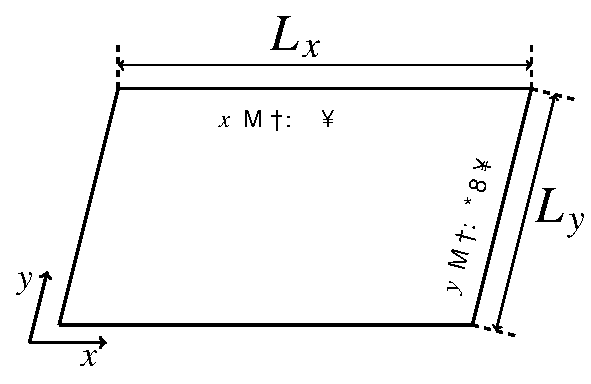
\includegraphics[scale=1]{figure1}
			\caption{考える系}
			\label{system}
		\end{figure}

	\section{問題}
		\subsection{ハミルトニアン $\mathcal{H}$ をフーリエ変換せよ}
		式(1)に式(8)を代入して計算していく。
		
		\begin{align}
			\mathcal{H}=\int \int \left( \frac{1}{\sqrt{L_y}}\sum_{k_y} \vec{\Psi}^\dagger _{k_y}(x) e^{-ik_yy} \right) \tilde{H} \left( \frac{1}{\sqrt{L_y}}\sum_{k_y'} \vec{\Psi}_{k_y'}(x) e^{ik_y'y} \right) dxdy
		\end{align}
		
		ここで
		
		\begin{align}
			\hat{\sigma}_0=
			\begin{bmatrix}
				1 & 0 \\ 
				0 & 1
			\end{bmatrix}
		\end{align}
		
		\begin{align}
			\hat{\sigma}_1=
			\begin{bmatrix}
				0 & 1 \\ 
				1 & 0
			\end{bmatrix}
		\end{align}
		
		\begin{align}
			\hat{\sigma}_2=
			\begin{bmatrix}
				0 & -i \\ 
				i & 0
			\end{bmatrix}
		\end{align}
		
		\begin{align}
			\hat{\sigma}_0=
			\begin{bmatrix}
				1 & 0 \\ 
				0 & -1
			\end{bmatrix}  
		\end{align}
		
		より、ハミルトニアン$\mathcal{H}$は、
		
		\begin{align}
			\mathcal{H}=
			\begin{bmatrix}
				-\frac{\hbar^2}{2m}\nabla^2-\mu_F & 0 & 0 & \Delta_0 \\ 
				0 & -\frac{\hbar^2}{2m}\nabla^2-\mu_F & -\Delta_0 & 0 \\ 
				0 & -\Delta_0^\ast & \frac{\hbar^2}{2m}\nabla^2+\mu_F & 0 \\ 
				\Delta_0^\ast & 0 & 0 & \frac{\hbar^2}{2m}\nabla^2+\mu_F
			\end{bmatrix} 
		\end{align}
		
		これを、式(9)に代入して計算していく。 \\
		このとき、
		
		\begin{align*}
			\vec{\Psi}_{k_y}^\dagger(x) e^{-ik_yy} \tilde{H}  \vec{\Psi}_{k_y'}(x) e^{ik_y'y} = 
			e^{-ik_yy} \left[ \Psi_\uparrow^\ast \left( -\frac{\hbar^2}{2m}\nabla^2-\mu_F \right) +\Psi_\downarrow^\ast \Delta_0^\ast \right] \Psi_\uparrow e^{ik'_yy} \\
			+e^{-ik_yy} \left[ \Psi_\downarrow^\ast \left( -\frac{\hbar^2}{2m}\nabla^2-\mu_F \right) -\Psi_\uparrow^\ast \Delta_0^\ast \right] \Psi_\downarrow e^{ik'_yy} \\
			+ e^{-ik_yy} \left[ -\Psi_\downarrow^\ast\Delta_0 +\Psi_\uparrow^\ast \left( \frac{\hbar^2}{2m}\nabla^2+\mu_F \right) \right] \Psi_\uparrow e^{ik'_yy} \\
			+e^{-ik_yy} \left[ \Psi_\uparrow^\ast\Delta_0 +\Psi_\downarrow^\ast \left( \frac{\hbar^2}{2m}\nabla^2+\mu_F \right) \right] \Psi_\downarrow e^{ik'_yy}
		\end{align*}
		
\end{document}
